% =====================================================================
%  DRAFT — fig-two-approaches-expanded.tex
%  NOT a final output. Source diagram for empirical-snapshot Option D
%  ("The Expanded Infographic"); see option-d-expanded-infographic.R.
%
%  Starts from the exact, already-approved "Two Approaches to Compliance"
%  diagram (papers/2026-epa-compliance-workshops/data-viz/code/
%  fig-two-approaches.tex) byte-for-byte, and extends the right-hand
%  arrow chain with one more linked box: the actual result, so the
%  standalone piece both poses the framing AND answers it, instead of
%  only setting up the question the way the research-highlight inset
%  does. The original diagram file is untouched -- this is a separate,
%  additive copy.
%
%  BUILD (from this folder):
%      pdflatex fig-two-approaches-expanded.tex
%  Then rasterize to PNG (pymupdf/fitz -- ghostscript is not installed
%  on this machine, only TinyTeX's rungs dispatcher stub):
%      python3 -c "
%      import fitz
%      doc = fitz.open('fig-two-approaches-expanded.pdf')
%      pix = doc[0].get_pixmap(dpi=300, alpha=True)
%      pix.save('../figures/fig-two-approaches-expanded.png')
%      "
%  option-d-expanded-infographic.R reads that PNG from ../figures/.
% =====================================================================
\documentclass[border=0pt]{standalone}
\usepackage[T1]{fontenc}
\usepackage[default]{sourcesanspro}
\renewcommand{\familydefault}{\sfdefault}
\usepackage{microtype}
\usepackage{tikz}
\usetikzlibrary{arrows.meta}

% ---- palette (identical to the original figure) ----------------------
\definecolor{maroon}{HTML}{8A2424}
\definecolor{graytext}{HTML}{6F6A63}
\definecolor{softgray}{HTML}{928D85}
\definecolor{leftfill}{HTML}{F0EFEC}
\definecolor{rightfill}{HTML}{F7EDEC}
\definecolor{rule}{HTML}{DDDDDB}

\begin{document}
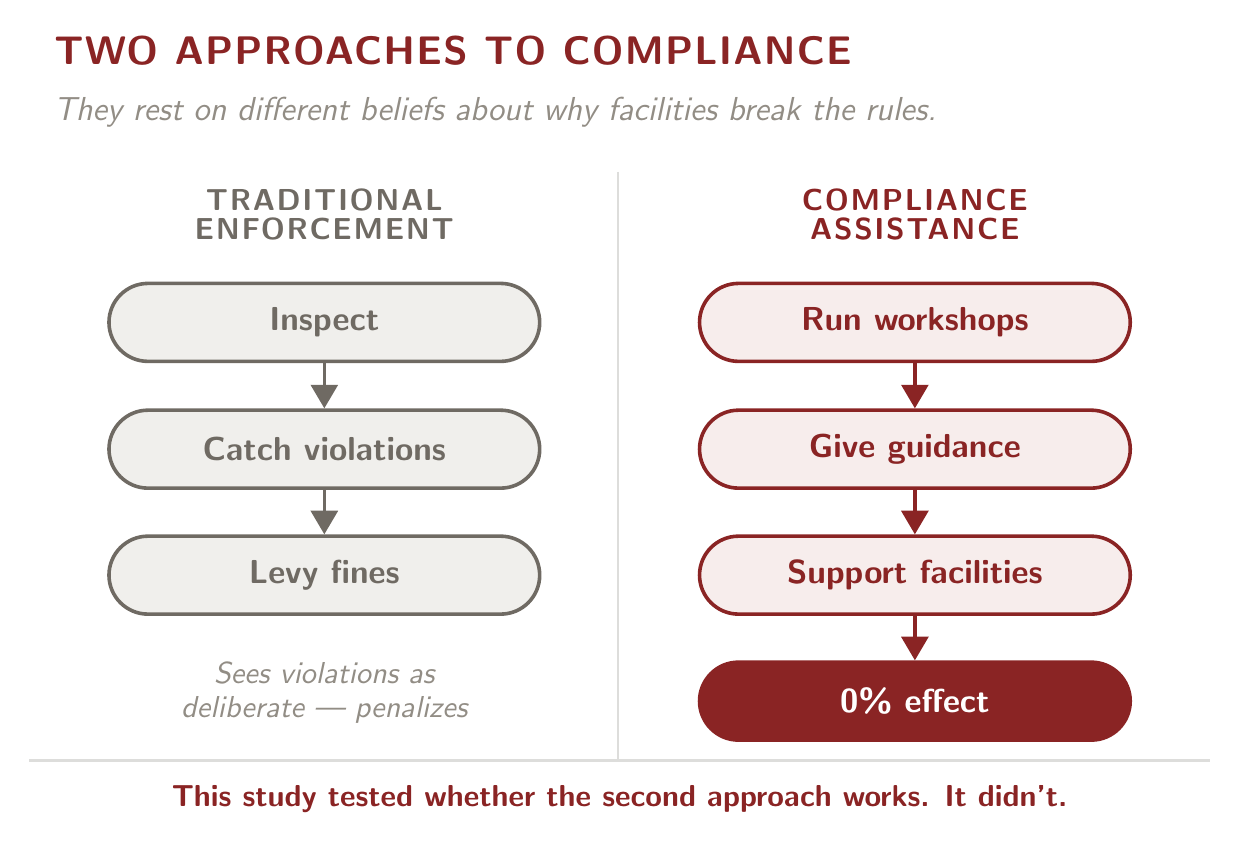
\begin{tikzpicture}[x=1mm,y=1mm,
  box/.style={rounded corners=4.95mm, minimum width=54.7mm,
              minimum height=9.9mm, line width=1.3pt, align=center,
              font=\bfseries\fontsize{11.5pt}{12pt}\selectfont},
  Lbox/.style={box, draw=graytext, fill=leftfill,  text=graytext},
  Rbox/.style={box, draw=maroon,   fill=rightfill, text=maroon},
  % Rresult: same size/shape as Rbox, but filled solid so it reads as the
  % "landing point" of the chain -- an outcome, not another action taken.
  Rresult/.style={box, draw=maroon, fill=maroon, text=white},
  Larr/.style={graytext, line width=1.3pt, -{Triangle[length=3mm,width=3.4mm]}},
  Rarr/.style={maroon,   line width=1.3pt, -{Triangle[length=3mm,width=3.4mm]}}]

  % =====================================================================
  % ORIGINAL DIAGRAM — unchanged from fig-two-approaches.tex, except the
  % right-hand chain gains one more linked box (the result) and its
  % caption is removed to make room -- see notes below.
  % =====================================================================
  \def\Lx{37.5}\def\Rx{112.5}
  \def\rowA{62.5}\def\rowB{46.4}\def\rowC{30.4}\def\rowD{14.4}

  \node[anchor=north west, maroon, font=\bfseries\fontsize{14pt}{15pt}\selectfont]
    at (1.9,100.0) {\textls[30]{TWO APPROACHES TO COMPLIANCE}};
  \node[anchor=north west, softgray, align=left,
        font=\itshape\fontsize{12pt}{13.5pt}\selectfont]
    at (1.9,92.3) {They rest on different beliefs about why facilities break the rules.};

  \node[graytext, align=center, font=\bfseries\fontsize{10.5pt}{11.5pt}\selectfont]
    at (\Lx,76.2) {\textls[50]{TRADITIONAL}\\[-0.2ex]\textls[50]{ENFORCEMENT}};
  \node[maroon, align=center, font=\bfseries\fontsize{10.5pt}{11.5pt}\selectfont]
    at (\Rx,76.2) {\textls[50]{COMPLIANCE}\\[-0.2ex]\textls[50]{ASSISTANCE}};

  \node[Lbox] (l1) at (\Lx,\rowA) {Inspect};
  \node[Lbox] (l2) at (\Lx,\rowB) {Catch violations};
  \node[Lbox] (l3) at (\Lx,\rowC) {Levy fines};
  \draw[Larr] (l1.south) -- (l2.north);
  \draw[Larr] (l2.south) -- (l3.north);

  \node[Rbox] (r1) at (\Rx,\rowA) {Run workshops};
  \node[Rbox] (r2) at (\Rx,\rowB) {Give guidance};
  \node[Rbox] (r3) at (\Rx,\rowC) {Support facilities};
  \draw[Rarr] (r1.south) -- (r2.north);
  \draw[Rarr] (r2.south) -- (r3.north);

  % --- NEW: the chain's fourth link -- what actually happened -----------
  % Same box size as the other three, so it reads as one more step in the
  % same process rather than a separate, differently-scaled callout. The
  % left column stops at three boxes because traditional enforcement
  % wasn't tested here -- there's nothing to add, so nothing is added.
  \node[Rresult] (r4) at (\Rx,\rowD) {0\% effect};
  \draw[Rarr] (r3.south) -- (r4.north);

  \node[anchor=north, softgray, align=center,
        font=\itshape\fontsize{11pt}{12.5pt}\selectfont]
    at (\Lx,20.6) {Sees violations as\\deliberate --- penalizes};

  \draw[rule, line width=1pt] (74.8,81.6) -- (74.8,6.9);

  \draw[rule, line width=1pt] (0,6.9) -- (150,6.9);
  \node[anchor=north, maroon, font=\bfseries\fontsize{10.7pt}{12pt}\selectfont]
    at (75,4.9) {This study tested whether the second approach works. It didn't.};

\end{tikzpicture}
\end{document}
